\documentclass[tikz, border=5mm]{standalone}

\usepackage{cmbright}

\usepackage{pgfplots}

% \kennlinie{soll}{niveau}{neigung}
\newcommand{\kennlinie}[4][]{\addplot [#1] {.55 * #4 * ((#2)^(x/(320-x * 4)))*((-x+20)*2)+ #2 + #3} node (x) [pos=0, right] {\scriptsize #2/#3/#4};}

\begin{document}
	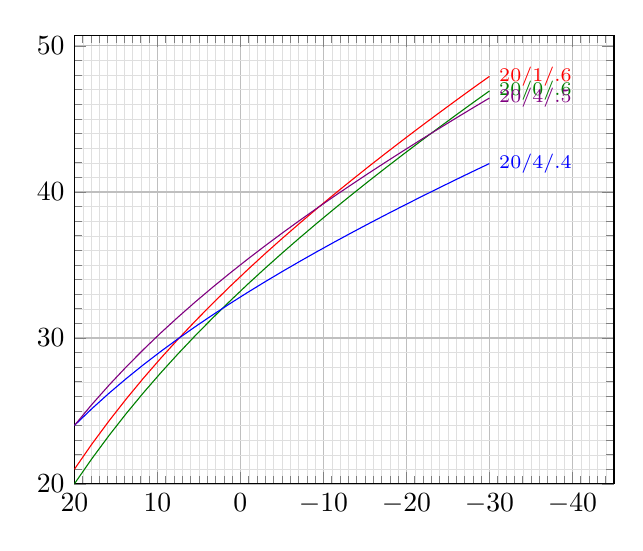
\begin{tikzpicture}
		\begin{axis}[domain=-30:20,
					 grid=both,
					 grid style={line width=.1pt, draw=gray!25},
					 major grid style={line width=.5pt, draw=gray!50},
					 minor tick num=9,
					 ymin=20,
					 xmin=-45,
					 xmax=20,
					 x dir=reverse,
					 ]
			\kennlinie[green!50!black]{20}{0}{.6};
			\kennlinie[red]{20}{1}{.6}
			\kennlinie[blue]{20}{4}{.4}
			\kennlinie[blue!50!red]{20}{4}{.5}
		\end{axis}
	\end{tikzpicture}
\end{document}
